
\renewcommand\appendixpagename{Anhänge}
\begin{appendices}


\chapter{Änderungen an der Parserdatei}
\begin{table}[h!]
    \centering
    \begin{tabular}{m{0.75cm}|m{4cm}|m{10cm}}
        \textbf{Zeile} & \textbf{Änderung} & \textbf{Begründung} \\
         \hline
        116 & Deklaration Kommentar & Hier wird ein mehrzeiliger Kommentar definiert, dies ist hier ein Alias für den Token \textit{JCOMMENT}\\
        \hline
        127-128 & \textit{comment} als mögliches Präfix in Klassenmember & Hier wird dem Parser mitgeteilt, dass ein Bestandteil einer Klasse wie z. B. eine Methode einen Javadoc-Kommentar besitzen kann\\
        \hline
        47 & \textit{comment} als mögliches Präfix vor Datentyp & Hier wird dem Parser mitgeteilt, dass ein Datentyp (Klasse, Schnittstelle etc. ) einen Javadoc-Kommentar haben kann \\
        \hline
        404 & Zulassung von Javadoc in Methoden & Da Javadoc-Kommentare an beliebigen Stellen auftauchen können, auch wenn es nicht empfohlen wird und keinen Mehrwert bietet, wird hier sichergestellt, dass solche Kommentare nicht zu Warnungen oder Fehler von ANTLR4 führen. Diese Javadoc-Kommentare werden nichtsdestotrotz später ignoriert.\\
        \hline
        34, 38& Zulassung von Kommentaren vor Paketdeklarationen und Imports & Hier werden Kommentare auch vor Paketdeklarationen und Import-Statements erlaubt, was vor allem bei Klassen mit Urheberrechtsangabe sinnvoll ist\\
        \hline
        105 & Zulassung von Kommentaren bei Enumerationen & Zwar werden Javadoc-Kommentare in Enumerationen mit diesem Tool nicht betrachtet, sie führen aber dennoch zu Warnungen und Fehlermeldungen. Daher werden sie hier zugelassen, aber später ignoriert. \\
        \hline
        82, 83 & Erzeugung eines separaten Knotens für \textit{Extends}- und \textit{Implements}-Deklarationen & In der originalen Version der Parserdatei wurde die Definition der Basisklasse bzw. der implementierten Schnittstellen direkt über die Tokens \textit{EXTENDS} bzw. \textit{IMPLEMENTS} gelöst. Dies wurde in einem neuen Knoten \textit{extendClass} bzw. \textit{implementInterfaces} ausgegliedert, um so das Parsing etwas zu vereinfachen.  \\
         
    \end{tabular}
    \caption{Änderungen an der Parserdatei}
    \label{tab:parser_changes}
\end{table}

\chapter{UML-Diagramm: Parser}
\begin{figure}[ht!]
\fontsize{5}{10}\selectfont
    \centering
    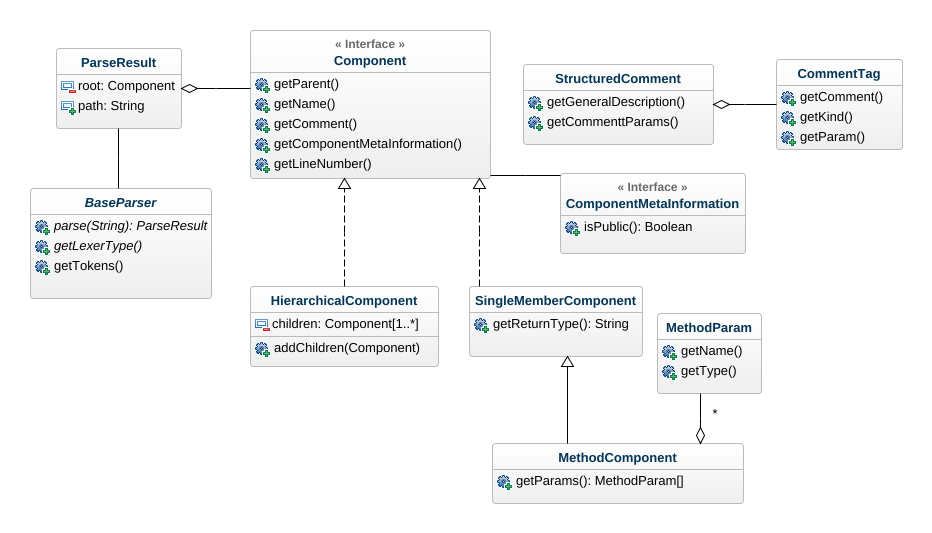
\includegraphics[height=9cm,keepaspectratio,angle=90]{figures/uml/parsing.png}
    \caption{UML-Diagramme aller Klassen, die relevant für das Parsen sind}
    \label{fig:uml_parsing}
\end{figure}
\chapter{UML-Diagramm: Metriken}
\begin{figure}[ht!]
\fontsize{5}{10}\selectfont
    \centering
    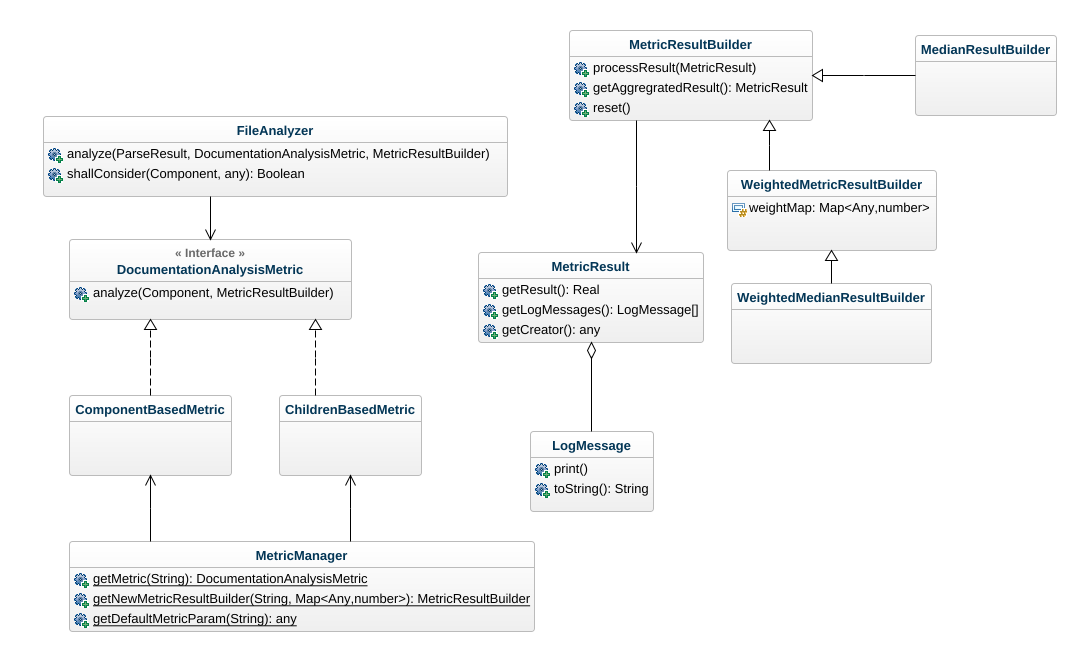
\includegraphics[height=10cm,keepaspectratio,angle=90]{figures/uml/metriken.png}
    \caption{UML-Diagramme aller Klassen, die relevant für die Metriken sind}
    \label{fig:uml_metrics}
\end{figure}
\chapter{Konfiguration des Tools}
\begin{description}
        \item[include]  Alle Dateien, die bei der Bewertung der Dokumentationsqualität berücksichtigt werden müssen
        \item[Exclude]  Teilmenge von include, enthält Dateien, die nicht weiter betrachtet werden müssen
        \item[metrics]  Alle Metriken, die das Tool verwenden soll. Dies ist ein Array von Objekten mit der Struktur \enquote{(name,weight,unique\_name,params)}, wobei \textit{weight} das Gewicht der jeweiligen Metrik ist( Bei Algorithmen ohne Relevanz des Gewichts wird es ignoriert), \textit{name} der Name (oder Aliasname) der Metrik und \textit{params} ein Objekt mit den Parametern der Metrik
        \item[absolute\_threshold] Mindestwert der Bewertung, die erreicht werden muss, sonst wird die Dokumentationsqualität nicht akzeptiert
       
          \item[builder] Der Algorithmus/\textit{ResultBuilder}, der die einzelnen Ergebnisse verarbeitet.
        
        \item[parser]  Kann verwendet, um die zu parsende Programmiersprache zu wählen. Dazu muss \textit{ParserFactory} angepasst werden
        
        \item[path\_weights] Ein Array von Objekten der Struktur \enquote{(path,weight)}. Wird verwendet, um einzelne Pfade höher oder niedriger zu gewichtet
        
         \item[component\_weights] Ein Array von Objekten der Struktur \enquote{(name,weight)}. Wird verwendet, um einzelne Komponenten höher oder niedriger zu gewichtet
         
         \item[default\_path\_weight] Das Standardgewicht für eine Datei, wenn keine passende Gewichtung gefunden wurde
         
         \item[default\_component\_weight] Das Standardgewicht einer Komponente, wenn keine passende Gewichtung gefunden wurde
         
         \item[state\_manager] Kann verwendet werden, um festzulegen, wie das letzte Ergebnis der Dokumentationsqualität gespeichert werden soll. Weitere Möglichkeiten können durch Erweiterung der \textit{StateManagerFactory} hinzugefügt werden.
         
         \item[relative\_threshold] Der maximale  relative Abstand zur letzten Dokumentationsqualität bevor eine Fehlermeldung geworfen wird.
        
        
        
    \label{enum:tool_javadoc_conf}
\end{description}
\chapter{Implementierte Metriken}\label{appendix_metrics}
\section{Anteil dokumentierter Komponenten an allen Komponenten}
\begin{description}
    \item [Metrikname]  simple\_comment
    \item [Klassenname] SimpleCommentPresentMetric
    \item[Beschreibung] Berechnet den Anteil der dokumentierten Komponenten an allen Komponenten, kann Getter und Setter ignorieren
\end{description}

\section{Anteil öffentlicher dokumentierter Komponenten an allen öffentlichen Komponenten}
\begin{description}
    \item [Metrikname]  public\_members\_only
    \item [Klassenname] SimplePublicMembersOnlyMetric
    \item[Beschreibung] Berechnet den Anteil der öffentlichen dokumentierten Komponenten an allen öffentlichen Komponenten, kann Getter und Setter ignorieren
\end{description}

\section{Bestrafung langer undokumentierter Methoden}
\begin{description}
    \item [Metrikname]  large\_method\_commented
    \item [Klassenname] SimpleLargeMethodCommentedMetric
    \item[Beschreibung] Bestraft undokumentierte Methoden je nach ihrer Länge
\end{description}

\section{Vollständigkeit der Dokumentation von Methoden}
\begin{description}
    \item [Metrikname]  method\_fully\_documented
    \item [Klassenname] SimpleMethodDocumentationMetric
    \item[Beschreibung] Prüft, ob alle Methodenparameter und Rückgabewert dokumentiert sind
\end{description}

\section{Anteil dokumentierter Methoden an allen Methoden unter
Berücksichtigung der LOC}
\begin{description}
    \item [Metrikname]  commented\_lines
    \item [Klassenname] CommentedLinesRatioMetric
    \item[Beschreibung]  Berechnet den Anteil der \ac{LOC} der dokumentierten Methoden an allen \ac{LOC} aller Methoden
\end{description}

\section{Kohärenz zwischen Kommentar und
Komponentenname}
\begin{description}
    \item [Metrikname]  comment\_name\_coherence
    \item [Klassenname] CommentNameCoherenceMetric
    \item[Beschreibung]  Prüft, ob der Kommentar und der Name der dokumentierten Komponente sehr ähnlich sind oder keine Ähnlichkeit haben, arbeitet nur mit Methoden
\end{description}

\section{Verwendung bestimmter Wörter bestrafen}
\begin{description}
    \item [Metrikname]  certain\_terms
    \item [Klassenname] CertainTermCountMetric
    \item[Beschreibung]  Bestraft das Vorkommen bestimmter Wörter (wie z.~B. Abkürzungen)
\end{description}

\section{Bewertung der Formatierung}
\begin{description}
    \item [Metrikname]  formatting\_good
    \item [Klassenname] FormattingGoodMetric
    \item[Beschreibung] Überprüft, ob korrekte Tags verwendet wurde, HTML-Tags geschlossen wurden und bei langen Methoden überhaupt eine Formatierung verwendet wurden
\end{description}


\section{Bewertung der Formatierung}
\begin{description}
    \item [Metrikname]  spellling
    \item [Klassenname] SpellingMetric
    \item[Beschreibung]Sucht nach Rechtschreibfehlern und bestraft sie
\end{description}

\section{Erwähnung von Randfällen bei Methodenparameter
und -rückgabewerte}
\begin{description}
    \item [Metrikname]  edge\_case
    \item [Klassenname] EdgeCaseMetric
    \item[Beschreibung] Prüft, ob bei der Dokumentation von Parametern die Behandlung des Wertes \textit{null} erwähnt wird
\end{description}


\section{Gunning-Fog-Index}
\begin{description}
    \item [Metrikname]  gunning\_fog
    \item [Klassenname] GunningFogMetric
    \item[Beschreibung] Berechnet den Gunnin-Fog-Index des Kommentars und bewertet so, ob der Kommentar verständlich ist
\end{description}
 

\begin{comment}
\begin{table}[ht!]
    \centering
    \begin{tabular}{m{4.5cm}|m{6.8cm}|m{5cm}}
        \textbf{Metrikname} & \textbf{Klassenname} & \textbf{Beschreibung}  \\\hline
          simple\_comment & SimpleCommentPresentMetric & Berechnet den Anteil der dokumentierten Komponenten an allen Komponenten\\\hline
        public\_members\_only & SimplePublicMembersOnlyMetric &   Berechnet den Anteil der öffentlichen dokumentierten Komponenten an allen öffentlichen Komponenten\\\hline
        large\_method\_commented & SimpleLargeMethodCommentedMetric & Bestraft undokumentierte Methoden je nach ihrer Länge\\\hline
     method\_fully\_documented & SimpleMethodDocumentationMetric & Prüft, ob alle Methodenparameter und Rückgabewert dokumentiert sind\\\hline
       commented\_lines\_ratio& CommentedLinesRatioMetric & Berechnet den Anteil der \ac{LOC} der dokumentierten Methoden an allen \ac{LOC} aller Methoden\\\hline
       flesch& FleschMetric & Berechnet den Flesch-Score des Kommentars und bewertet so, ob der Kommentar verständlich ist\\\hline
        comment\_name\_coherence&CommentNameCoherenceMetric & Prüft, ob der Kommentar und der Name der dokumentierten Komponente sehr ähnlich sind oder keine Ähnlichkeit haben\\\hline
     certain\_terms&CertainTermCountMetric & Bestraft das Vorkommen bestimmter Wörter (wie z.~B. Abkürzungen)\\\hline
          formatting\_good&FormattingGoodMetric & Überprüft, ob korrekte Tags verwendet wurde, HTML-Tags geschlossen wurden und bei langen Methoden überhaupt eine Formatierung verwendet wurden\\\hline
          spellling&SpellingMetric & Sucht nach Rechtschreibfehlern und bestraft sie\\\hline
        edge\_case&EdgeCaseMetric & Prüft, ob bei der Dokumentation von Parametern die Behandlung des Wertes \textit{null} erwähnt wird\\\hline
        gunning\_fog&GunningFogMetri& Berechnet den Gunnin-Fog-Index des Kommentars und bewertet so, ob der Kommentar verständlich ist\\
    \end{tabular}
    \caption{Alle implementierten Metriken}
    \label{table:metrics_name}
\end{table}
\end{comment}

\chapter{Rohdaten der Geschwindigkeitsmessung}\label{chapter:raw_speed_data}
\begin{table}[]
    \centering
    \begin{tabular}{c|c|c}
DE & CS &PMD\\\hline
2.633 &	2.483&	1.824\\\hline
		
2.640&	2.458&	1.807\\\hline
		
2.544&	2.315&	2.007\\\hline
		
2.533&	2.260&	1.971\\\hline
		
2.602&	2.285&	1.882\\\hline
		
2.404&	2.275&	2.024\\\hline
		
2.514&	2.645&	1.942\\\hline
		
2.412&	2.239&	1.917\\\hline
		
2.579&	2.744&	1.890\\\hline
		
2.522&	2.215&	1.897\\\hline
  \end{tabular}
    \caption{Benötigte Zeitdauer bei Log4J in Sekunden}
    \label{tab:raw_log4j}
\end{table}


\begin{table}[]
    \centering
    \sisetup{round-mode=places,round-precision=3}
    \begin{tabular}{c|c|c}
DE & CS &PMD\\\hline

16.719&	9.384&	8.036\\\hline
		
17.111&	9.431&	7.631\\\hline
		
16.715&	9.212&	7.658\\\hline
		
17.089&	9.414&	8.197\\\hline
		
16.486&	9.169&	7.985\\\hline
		
16.934&	9.303&	7.918\\\hline
		
17.003&	9.387&	7.884\\\hline
		
17.033&	9.269&	7.913\\\hline
		
16.997&	9.299&	7.916\\\hline
		
16.712&	9.268&	7.944\\\hline
    \end{tabular}
    \caption{Benötigte Zeitdauer bei ArgoUML in Sekunden}
    \label{tab:raw_argo}
\end{table}


\begin{table}[]
    \centering
    \begin{tabular}{c|c|c}
DE & CS &PMD\\\hline
69.867&27.581&22.235\\\hline
69.179&27.439&21.843\\\hline
69.118&27.849&21.738\\\hline
69.038&27.285&21.594\\\hline
68.620&27.079&21.561\\\hline
68.409&27.216&21.451\\\hline
69.765&27.346&21.178\\\hline
74.260&27.226&21.577\\\hline
70.197&27.239&21.558\\\hline
69.018&27.909&21.880\\\hline
    \end{tabular}
    \caption{Benötigte Zeitdauer bei Eclipse JDT in Sekunden}
    \label{tab:raw_eclipse}
\end{table}
\chapter{Boxplots: Geschwindigkeitsevaluation}\label{appendix:boxplots}
Nachfolgend werden die Boxplots aus Kapitel \ref{chapter:eval_speed_result} in vergrößerter Darstellung aufgeführt:
 \begin{figure}[ht!]
\includesvg[width=0.96\textwidth]{figures/chapter5/log4j_speed_boxplot.svg}
    \caption{Boxplot: Log4J}
  
\end{figure}
\hfill
 \begin{figure}
    \centering
\includesvg[width=\textwidth]{figures/chapter5/argo_speed_boxplot.svg}
    \caption{Boxplot: ArgoUML}
  
\end{figure}

 \begin{figure}
    \centering
\includesvg[,width=\textwidth]{figures/chapter5/eclipse_speed_boxplot.svg}
    \caption{Boxplot: Eclipse \ac{JDT} }
  
\end{figure}
\end{appendices}
	
